\Chapter{A lekérdezőnyelv}

\section{Alaptípusok}

\begin{itemize}

\item Boolean: Logikai adattípus.
 Ha paraméter nélkül hozzuk létre, akkor autómatikusan false értéket ad az adatbázisban tárolt adatok listájához.

\begin{sql}
INSERT Boolean() INTO azeroth;
INSERT Boolean(true) INTO azeroth; 
INSERT Boolean(false) INTO azeroth;
INSERT Boolean(SELECT bool FROM azeroth WHERE bool IS Boolean AND bool.id = "bool11") INTO azeroth;
\end{sql}



\begin{figure}[htb]
\begin{center}
    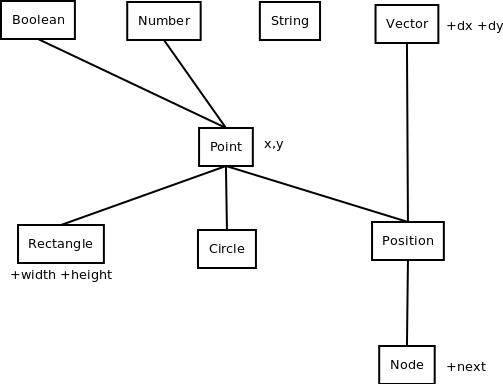
\includegraphics[scale=0.5]{images/types}
    \caption{A lekérdezőnyelv alaptípusai}
    \label{fig:types}
\end{center}
\end{figure}

\item Number: Valós vagy egész szám 4 byteon való tárolására alkalmas
\begin{sql}
INSERT Number(1.2) INTO azeroth;
INSERT Number(12) INTO azeroth;
INSERT Number(SELECT number FROM azeroth WHERE number IS Number AND number.id = "numberasd11") INTO azeroth; /*Ez egy másik Number objektumra mutat.*/
INSERT Number(SELECT number FROM azeroth WHERE number HAS x AND number.x IS Number AND number.id = "num11") INTO azeroth;
\end{sql}

Itt azt csinálom, hogy olyan Number objektumot adok a térképhez, ami a num11 id-jű elem(ez lehet akár mine is) x attribútumára mutat, tehát ha az megváltozik, akkor ez az újonnan hozzáadott Number is megfog arra változni.

\begin{sql}
INSERT Number(Number(11)) INTO azeroth;
\end{sql}

\item String: Szöveg tárolása.

\begin{sql}
INSERT String("alma") INTO azeroth;
INSERT String(SELECT string FROM azeroth WHERE string IS String AND string.id="stringasd11") INTO azeroth;
INSERT String(String("körte")) INTO azeroth;
\end{sql}

Ez a megoldás is járható út, hisz a String("alma") kifejezés az visszatér egy új String példánnyal, aminek az értéke „alma".

\item Vector: Irány tárolását teszi lehetővé.

\begin{sql}
INSERT Vector(10, 20) INTO azeroth;
INSERT Vector(Number(10), Number(20)) INTO azeroth;
INSERT Vector(Number(10), 20) INTO azeroth;
INSERT Vector(10, Number(20)) INTO azeroth;
INSERT Vector(SELECT vector FROM azeroth WHERE vector IS Vector AND vector.id="vetorasd11") INTO azeroth;
\end{sql}

Ilyenkor egy másik Vector objektumra hivatkozik, tehát ha annak az értéke változik valamelyik a kettő közül, akkor ennek is fog.

\begin{sql}
INSERT Vector(SELECT number FROM azeroth WHERE number is Number AND number.id = "numasd11", 10) INTO azeroth;
\end{sql}

Ilyenkor a vector dx attribútuma egy másik Number objektumra mutat, tehát ha az változik, akkor ez is fog.

\begin{sql}
INSERT Vector(SELECT number FROM azeroth WHERE number is Number AND number.id = "numasd11", SELECT number FROM azeroth WHERE number is Number AND number.id = "numasd12") INTO azeroth;
\end{sql}

Itt mind a két attribútuma más Number objektumra mutat, viszont ez is járható út.

\begin{sql}
INSERT Vector(Vector(10, 20)) INTO azeroth;
\end{sql}

\item Point: Egy pont, melynek nincs iránya. Két Number típust tartalmaz(x,y).

\begin{sql}
INSERT Point(10, 20) INTO azeroth;
INSERT Point(Number(10), Number(20)) INTO azeroth;
INSERT Point(Number(10), 20) INTO azeroth;
INSERT Point(10, Number(20)) INTO azeroth;
INSERT Point(SELECT point FROM azeroth WHERE point IS Point AND point.id="pointasd11") INTO azeroth;
\end{sql}

Ilyenkor egy másik Point objektumra hivatkozik, tehát ha annak az értéke változik valamelyik a kettő közül, akkor ennek is fog.

\begin{sql}
INSERT Point(SELECT number FROM azeroth WHERE number is Number AND number.id = "numasd11", 10) INTO azeroth;
\end{sql}

Ilyenkor a point x attribútuma egy másik Number objektumra mutat, tehát ha az változik, akkor ez is fog.
\begin{sql}
INSERT Point(SELECT number FROM azeroth WHERE number is Number AND number.id = "numasd11", SELECT number FROM azeroth WHERE number is Number AND number.id = "numasd12") INTO azeroth;
\end{sql}

Itt mind a két attribútuma más Number objektumra mutat, viszont ez is járható út.
\begin{sql}
INSERT Point(Point(10, 10)) INTO azeroth;
\end{sql}

\item Dimension: Egy szélesség és egy magasság number értéket tárol.
\begin{sql}
INSERT Dimension(10, 20) INTO azeroth;
INSERT Dimension(Number(10), Number(20)) INTO azeroth;
INSERT Dimension(Number(10), 20) INTO azeroth;
INSERT Dimension(10, Number(20)) INTO azeroth;
INSERT Dimension(SELECT dimension FROM azeroth WHERE dimension IS Dimension AND dimension.id="dimensionasd11") INTO azeroth;
\end{sql}

Ilyenkor egy másik Dimension objektumra hivatkozik, tehát ha annak az értéke változik valamelyik a kettő közül, akkor ennek is fog.

\begin{sql}
INSERT Dimension(SELECT number FROM azeroth WHERE number is Number AND number.id = "numasd11", 10) INTO azeroth;
\end{sql}

Ilyenkor a dimension width attribútuma egy másik Number objektumra mutat, tehát ha az változik, akkor ez is fog.

\begin{sql}
INSERT Dimension(SELECT number FROM azeroth WHERE number is Number AND number.id = "numasd11", SELECT number FROM azeroth WHERE number is Number AND number.id = "numasd12") INTO azeroth;
\end{sql}

Itt mind a két attribútuma más Number objektumra mutat, viszont ez is járható út.
\begin{sql}
INSERT Dimension(Dimension(10,10)) INTO azeroth;
\end{sql}

Ezzel a fenti példájára ugyan így megadható.

\item Rectangle: Téglalap tárolására szolgál.Tatralmaz egy Pointot, amiben tárolja a bal felső sarkának koordinátáit, illetve egy Dimensiont, melyek a szélesség és magasság attribútumok lesznek.

\begin{sql}
INSERT Rectangle(Point(10,10), Dimension(100, 200)) INTO azeroth;
INSERT Rectangle(Rectangle(10, 10, 100, 100)) INTO azeroth;
\end{sql}

Itt az a lényeg, hogy lehet belül azzal a new nélküli kifejezéssel is visszaadatni új objektumot.

\begin{sql}
INSERT Rectangle(10, 10, 100, 200) INTO azeroth;
INSERT Rectangle(10, 10, Dimension(100, 200)) INTO azeroth;
INSERT Rectangle(Point(10, 10), 100, 200) INTO azeroth;
INSERT Rectangle(SELECT rectangle FROM azeroth WHERE rectangle IS Rectangle AND id = "rectasd11") INTO azeroth;
INSERT Rectangle(SELECT number FROM azeroth WHERE number is Number AND number.id = "numasd11", SELECT number FROM azeroth WHERE number is Number AND number.id = "numasd12", SELECT number FROM azeroth WHERE number is Number AND number.id = "numasd13", SELECT number FROM azeroth WHERE number is Number AND number.id = "numasd14") INTO azeroth;
\end{sql}

Itt mind a 4 paraméter egy lekérdezés eredménye, azaz mind mutat valamire.
Attól függetlenül, hogy hozzuk létre a Rectangle-t(4 paraméterrel vagy máshogy),  ez tárolni egy Pointban és egy Dimensionben fogja.

\item Circle: Még egyeztetés alatt a létjogosultsága.


\item Position: Ez egy olyan pont, aminek van iránya. Egy pont és egy vector.
\begin{sql}
INSERT Position(Point(10, 10),  Vector(100, 100)) INTO azeroth;
INSERT Position(Position(10, 10, 100, 100)) INTO azeroth;
\end{sql}

Itt az a lényeg, hogy lehet belül azzal a new nélküli kifejezéssel is visszaadatni új objektumot.

\begin{sql}
INSERT Position(10, 10, 100, 200) INTO azeroth;
\end{sql}
Ilyenkor a sorrend x,y,dx,dy.
\begin{sql}
INSERT Position(10, 10, Vector(100, 200)) INTO azeroth;
INSERT Position(Point(10, 10), 100, 200) INTO azeroth;
INSERT Position(SELECT position FROM azeroth WHERE position IS Position AND id = "posasd11") INTO azeroth;
INSERT Rectangle(SELECT number FROM azeroth WHERE number is Number AND number.id = "numasd11", SELECT number FROM azeroth WHERE number is Number AND number.id = "numasd12", SELECT number FROM azeroth WHERE number is Number AND number.id = "numasd13", SELECT number FROM azeroth WHERE number is Number AND number.id = "numasd14") INTO azeroth;
\end{sql}

Itt mind a 4 paraméter egy lekérdezés eredménye, azaz mind mutat valamire.

\item Node: Olyan Position, ami tartalmaz egy referenciát a következő Nodera. Ezzel egy láncolt Nodeok halmazát kapjuk, a sorrendiség adott a láncolt listából, hisz mindegyik Node az utána következőre mutat. Ezzel felírható egy egyenes, vagy útvonal. 
INSERT Node(Node(10, 10, 100, 100, NULL)) INTO azeroth; 

Itt úgy hozunk létre Nodeot, hogy a szimpla kifejezéssel, és a NULL az azt jelenti, hogy ő már nem mutat további Nodera, lehet hogy rá sem mutat semmi, akor ez egyenlőre egy szimpla Positionként funkcionál.

\begin{sql}
INSERT Node(10, 10, 100, 100, NULL) INTO azeroth;
INSERT Node(10, 10, 100, 100, SELECT node FROM azeroth WHERE node IS Node AND node.id = "nodeasd11") INTO azeroth;
\end{sql}
Itt már úgy hozunk létre egy Nodeot, hogy az egy másik Nodera mutat, egy már létező Node objektumra.
\begin{sql}
INSERT Node(10, 10, 100, 100, Node(200, 200, 2000, 2000, NULL)) INTO azeroth;
\end{sql}
Ez a megoldás is járható út, ilyenkor a belső Node objektumra fog mutatni, ami viszont ilyenkor még nincs a mapen, de ez így hozzáteszi azzal, hogy ő hivatkozik rá a láncban.
\begin{sql}
INSERT Node(10, 10, 100, 100, NULL, true) INTO azeroth;
\end{sql}
Ha 5. paraméternek beírunk egx truet, akkor azt jelenti, hogy ez egy Lánc első eleme, innen indul ki az összes többi(Ha az utolsó elem erre mutat, akkor kapunk egy körutat.)
\begin{sql}
INSERT Node(10,10, 100, 100, NULL, false) INTO azeroth;
\end{sql}
Így is létrehozható egy Node, ez az alapértelmezett, tehát ha nem tüntetjük fel, hogy false, akkor alapértelmezés szerint false lesz annak a booleannak az értéke, ami azt jelzi, hogy ez a Node olyan-e, amiből kiindul egy út.
\begin{sql}
INSERT Node(10,10, 100, 100) INTO azeroth;
\end{sql}
Ha elhadjuk azt a paramétert, ami a következő Nodera mutatna, akkor azzal sincs semmi gond, mert az autómatikusan beilleszti oda a NULL értéket.

\item Path: Node-ok halmaza.

\begin{sql}
INSERT Path(Node(10,10,10,10), Node(10,20), Node(10,10,100,35)) INTO azeroth;
\end{sql}

Itt az útvonal úgy jön létre, hogy a paraméterlistában szereplő Nodeokat úgy hozza létre, hogy paraméterlistában való elhelyezkedés szerint adja értékül a next értéknek mindig a következőt. Az utolsó elem NULL- ra mutat. Az első elemre ha nem körútról van szó , akkor nem mutat semmi. Minden Node objektumnak van egy isFirst Boolean attribútuma, ami csak az első elemnek vesz fel true értéket, hogy tudjuk honnan indul az útvonal. Ez az isFirst a Path létrehozási mechanizmusban autómatikusan kap értéket, erről a felhasználónak nem kell gondoskodnia.
Látható, hogy az egyik Node-ot kevesebb(mindössze kettő paraméterrel) hoztuk létre. Ez nem jelent semmi problémát, ilyenkor az irány nincs megadva, de arra nem is feltétlenül van szükség.
A Node adattípus leírásánál elmondtuk, hogy Node(10,10,10,10) létrehozva úgy, hogy nem adjuk meg a következő Nodera mutató elemet, akkor az autómatikusan NULL lesz, viszont ha ez Path() inicializálásnál történik, akkor a Path inicializálás ad neki értéket.

\begin{sql}
INSERT Path(SELECT node FROM azeroth WHERE node IS Node AND node.id = "nodeasd11") INTO azeroth;
\end{sql}

Egy Path nem hozható létre úgy, hogy  meglévő Nodeok összegyűjtéséből. Tehát a Path inicializálásnál nem szerepelhet egyetlen Select sem, mert az hibát jelent.

Egy objektum ha referenciát tartalmaz egy másik objektumra akkor az eléri bármikor a hivatkozottat, viszont a hivatkozott nem tud hivatkozni arra aki rá hivatkozik, erre nincs nyelvi elem definiálva, hisz szükségtelen, nagyon kevés alkalmazhatósága lenne, így kimaradt a lekérdező nyelv készletéből.

Mit követeljünk meg number x, number y vagy Point xy ?
Ha van x,y numbere, vagy location Point vagy Position attribútuma a user által definiált classnak, akkor végezhető vele distanceFrom, Collide, stb...

\end{itemize}

\section{Támogatott operátorok}
\begin{itemize}
\item = 
\item <= 
\item >= 
\item > 
\item < 
\item <> (nem egyenlő) 
\item OR 
\item AND 
\item IS 
\item COLLIDE
\item NOT
\end{itemize}

A fenti operátorok boolean értékkel térnek vissza.

Lássunk mindegyikre egy példát:
\begin{sql}
SELECT mine FROM azeroth WHERE mine.id = "asd11";
SELECT mine FROM azeroth WHERE mine.x <= 10;
SELECT mine FROM azeroth WHERE mine.y >= 10;
SELECT mine FROM azeroth WHERE mine.x <> 20;
\end{sql}

A mine.x jelölés rejtve azt a feltételt is jelenti, hogy mine HAS x , és ez AND kapcsolattal jön hozzá.
\begin{sql}
SELECT mine FROM azeroth WHERE mine.stone.location.x > 10;
\end{sql}

Olyan objektumokat kérdez le, amiknek van stone attribútuma, aminek van location attribútuma, aminek van x attribútuma(ezeket mind HAS-sal megvuszgáljuk, és ennek az x attribútumnak az értéke nagyobb mint 10.)
\begin{sql}
SELECT mine FROM azeroth WHERE mine IS Mine;
\end{sql}
Az IS operátor az objektum típusának ellenőrzésére szolgál, az IS bal odlalán egy szimbólum, jobb oldalán pedig egy Class név kell szerepeljen.
\begin{sql}
SELECT mine FROM azeroth WHERE mine.x = 10 AND mine.y < 20;
\end{sql}

A logikai műveletek a WHERE után kombinálhatóak is természetesen:
\begin{sql}
SELECT mine FROM azeroth WHERE mine.x = 10 AND mine.y = 20 OR mine.id=100;
\end{sql}
Ha nincs zárójelezés, akkor sorban veszi a feltételeket.
\begin{sql}
SELECT mine FROM azeroth WHERE mine.x = 10 AND (mine.y = 20 OR mine.id = 100);
\end{sql}

\begin{sql}
SELECT mine FROM azeroth WHERE mine.x = 10 AND NOT (mine.y = 20 OR mine.id = 100 OR 10=10);
\end{sql}
Azokat a mineokat gyűjti ki, amelyek x attribútuma 10, és y attribútuma nem egyenlő 20, és az id-jük nem egyenlő 100-al.
\begin{sql}


Azokat a mineokat választja ki, amelyek nem a legközelebb helyeszkednek el a 10,10 ponthoz.
\begin{sql}
SELECT mine FROM azeroth WHERE mine NOT COLLIDE POINT(10, 10);
\end{sql}
Azokat a mineokat választja ki, amelyek nem tartalmazzák a 10, 10 pontot.


A kiértékelésben a zárójelnek szerepe lehet, ezt az eszközt a felhasználó kezébe adja az adatbázis.

\section{Saját osztályok definiálása}

\section{Metódusok}

Metódusok a lekérdező nyelvben

Csak a gyárilag definiált osztályok rendelkeznek metódusokkal(Boolean,Number,Vector,Rectangle,stb.).
Ezek gyári szolgáltatások az adott adattípushoz.Viszont amikor a felhasználó készít saját Osztálydefiníciót, ő csak adatleírást végezhet, metódusokat nem definiálhat hozzájuk.A gyárilag elkészített metódusok a típusokhoz valamely szolgáltatást jelentenek.Dimension tud területet számítani magán, a Vector tud szöget számítani, a Rectangle megtudja mondani, hogy Collided vele egy másik Rectangle, illetve sok definiált metódusuk van. Ezeket itt folytatni kell……….!!!!!!!!!!!!!!!!!!!!!!! 

\section{DDL adatdefiníciós utasítások}

CREATE: Létrehozó parancs, mellyel objektumokat vagy classokat lehet létrehozni.
CREATE DATABASE db;
CREATE MAP azeroth; /*Létrehoz egy azeroth nevezetű mapet a jelenlegi adatbázisban.*/
CREATE CLASS Mine; /*Definiál egy Mine classt a jelenlegi adatbázisba.*/
Az adatbázis fogja össze a Mapeket. 
-CREATE CLASS Mine; /*Ilyenkor létrehozy egy mine classt, az alap attribútumokkal.*/
- CREATE CLASS Mine(
	Number age,
	String name,
	Number x,
	Number y,
);  /*Autómatikussan minden insertkor beillesztődik egy id attribútum érték nekik. A definiált classokba van id attribútum, azt nem kell definiálni, boolean stringbe alapból nincs beillesztve, azoknak értelmetéen lenne adni, tehát a definiált alaptípusoknak nincs id attrubútumuk.*/

Amikor definiálunk egy osztályt, akkor nincs lehetőségünk öröklődésre, mint például Javaban, itt kompozíciót lehet alkalmazni ezen célra.
A Classok természetesen tartalmazhatnak attribútumként más classokat is:

\begin{sql}
CREATE CLASS Mine(
	Stone stone,  /*Stone eobjektumot tartalmaz*/
	Number size,
);

CREATE CLASS Mine(
	Number kor DEAFAULT 18,
);
\end{sql}

DEFAULT jelző, ha nem kap értéket Inserteléskor, akkor ez szúródik be neki.DEFAULT jelző csak primitív típusok mellett szerepelhet(String, Number,Boolean).

A MAP-eket is az adatbázis, és a CLASS-okat is az adatbázis fogja össze. Tehát a CLASS-okat nem MAP-ekhez hozzuk létre, hanem adatbázisokhoz.

Az id-k autómatikus kiosztása úgy történik, hogy minden Map-en külön számláló van erre a célra. Azaz azeroth mapen is van 0 id-jű elem, és og mapen is.A Map-ek elemei nem keveredhetnek.


-DROP: Elvet egy objektumot vagy osztályt.
\begin{sql}
DROP DATABASE db1;
DROP MAP azeroth;
\end{sql}
A két fenti utasítás értelemszerűen törlést visz végbe. Ha törlök egy adatbázist, akkor minden benne lévő elem törlődik(Class definíciók, Mapek, mentések).
Ha törlök  egy Mapet, akkor minden benne tárolt elem törlődik vele együtt.

\begin{sql}
DROP CLASS Mine;
\end{sql}
Osztálydefiníció megszüntetése. Csak olyan osztálydefiníciót lehet megszüntetni, amire nincs hivatkozás, azaz egyik mapen sincs belőle példány létrehozva.

-ALTER: Szerkezetmódisító művelet. 
Szerkezete módosítani csak az osztálydefinícióknak lehet. Ennek négy típusa van:


\begin{sql}
ALTER CLASS Mine ADDATTRIBUTE name String;
\end{sql}
Csak azoknál az osztályoknál lehet szerkezetet módosítani, amelyekből egyetlen példány sincs létrehozva az adatbázisban.

\begin{sql}
ALTER CLASS Mine RENAMEATTRIBUTE size TO name;
\end{sql}
Át lehet nevezni egy attribútumot, innentől kezdve ezen a néven lehet rá hivatkozni.

\begin{sql}
ALTER CLASS Mine DELETEATTRIBUTE size;
\end{sql}
Törli a size attribútumát ennek a Mine Class definíciónak.

\begin{sql}
ALTER CLASS Mine RENAMECLASS BigMine;
\end{sql}
Az osztály nevének megváltoztatása.

\section{DML adatkezelő utasítások}

DELETE: Objektum törlés. Objektum alatt létrehozott Class példányokat értjük.

\begin{sql}
DELETE mine FROM azeroth WHERE  mine IS Mine;
\end{sql}
Az összes Mine típusú elemet kitörli az azeroth térképről.
\begin{sql}
DELETE mine FROM azeroth;
\end{sql}
/*Minden elemet kitöröl a térképről*/
\begin{sql}
DELETE object FROM azeroth WHERE object HAS x;
\end{sql}
Minden elemet kitöröl az azeroth térképről, aminek van x attribútuma.

-UPDATE: Objektum tartalom módosítás.
\begin{sql}
UPDATE azeroth SET x = 30 WHERE id="asd11";
\end{sql}
Az azeroth térképen lévő asd11 elem x attribútumának értékét 30-ra állítja ütközésvizsgálat nélkül.

\begin{sql}
UPDATE azeroth MOVE  mine TO  (10,10) WHERE mine.id = "asd11";
\end{sql}
Azt mozgatja el, akinek van id tulajdonsága és az asd11". Ebben a verzióban a (10,10) pontba toljuk az objektumot.
\begin{sql}
UPDATE azeroth MOVE  mine.x TO 10 WHERE mine.id = "asd11";
\end{sql}
Azt mozgatja el, akinek van id tulajdonsága és az asd11. Ebben a megoldásban csak egy attribútum szerinti változtatás történik, tehát az új pozíció ahova rakjuk az elemet, az x = 10, és az y pedig maradt ami volt.
\begin{sql}
UPDATE azeroth MOVE  mine BY  (10,10) WHERE mine.id = "asd11";
\end{sql}
Azt mozgatja el, akinek van id tulajdonsága és az asd11. Ebben a megoldásban egy vector segítségével toljuk el az objektumot, tehát nem új pozíciót adunk meg, hanem elmozdulási irányt és mértéket.

Látható, hogy két -féle UPDATE művelet létezik az adatbázisban. Az egyik, amikor a set kulcsszó szerepel, akkor mindenféle ütközésvizsgálat nélkül bármely attribútum értékét változtathatjuk az adott objektumnak, nincs megkötés, hogy csak pozíciót lehetne.

A másik amikor a MOVE kulcsszó is szerepel a lekérdezésben, ott bizony ütközésvizsgálattal egybekötött paraméter értékváltoztatás történik. Ott igazából  csak x,y koordináták változtathatóak.

Az UPDATE lekérdezés különlegessége, hogy visszaadja a módosított elemek halmazát.

-Insert: Új objektum felvétele egy térképre. 
Nem lehet úgy létrehozni objektumot, hogy nem adunk minden attribútumának értéket.
Az ADD-nél szükség van egy olyan környezeti változóra, ami azt tartalmazza, hogy a most beszúrt elemek mely z-index szintre szúrja be a mostani elemeket.
A LAYER 1 azt jelenti, hogy a beszúrandó elemek zlayer attribútumát 1-re állítja, a zindexet, pedig az első szinten lévő következő indexre(ezt a háttérben egy vektorban tároljuk, hogy mely layeren mi az aktuálisan kiosztandó zindex szám.)
\begin{sql}
ADD Szobor(location,name) INTO azeroth VALUES(Point(10,10), "asdJani") LAYER 1;
\end{sql}
Itt létrehozunk egy új Szobor példányt az azeroth térképre.

\begin{sql}
INSERT Mine(x, Stone(Location(x,y), w, h), age) INTO azeroth Values(10, Stone(Location(10, 20), 30, 40), 1234);
\end{sql}
Látható, hogy a values is elég rendesen egymásba ágyazható.

Megadható, hogy mely attribútumoknak fogunk értéket adni inserteléskor.
\begin{sql}
ADD Szobor(x,y,stone(x,y),name) INTO azeroth VALUES(10,10,(10,20),"name");
\end{sql}
Ennek a példának az a különlegessége, hogy példányosításban példányosítunk.

\begin{sql}
ADD Szobor INTO azeroth VALUES(10,10,(,20,20),"asd",123);
\end{sql}
Ilyenkor, amikor nem adjuk meg zárójelek között, hogy mely attribútumainak szeretnénk inicializáló értéket adni, ilyenkor mindnek kell.

Fontos megemlíteni, hogy létrehozhatunk úgy objektumot, hogy az attribútumai között van olyan, aminek nem másolatot adunk, hanem referenciát, hogy arra mutasson.
\begin{sql}
ADD Szobor(x,y,stone(x,y)) INTO azeroth VALUES(10, 10, SELECT stone FROM azeroth WHERE stone IS Stone AND stone.id = "asd11");
\end{sql}
Látható, hogy itt ennek a szobornak egy stone attribútumba egy lekérdezés eredményét adom, ami egy létező objektum, tehát arra fog mutatni(id alapján).
Ha ennek a selectnek több értékű halmaz eredménye lesz, akkor hiba dobódik, mivel létrehozásnál egy elemet várunk.Ha üres halmazt kapunk, akkor sem történik meg a beszúrás, akkor is hiba keletkezik, akkor viszont jelzi, hogy nullértékű értékátadás történt.

\section{DQL lekérdező utasítások}

\begin{sql}
SELECT mine From azeroth;
\end{sql}
A mine egy kifejezés, amin keresztül elérhetjük az összes  azeroth mapen lévő objektumot. A Select után csak egy ilyen kifejezés állhat. Ez azt csinálja, hogy visszaad egy halmazt, amiben minden elem(point,rectangle,saját definiált class) benne van szűkítés nélkül.
\begin{sql}
SELECT mine.x from azeroth;
\end{sql}
Ez visszaadja azon elemek halmazát az azeroth mapről, melyeknek van x attribútumuk, és azoknak az attribútumoknak a halmazát adná(Tehát itt number x-ek lennének az eredmény halmazban.)


\begin{sql}
Min(SELECT mine.x from azeroth);
\end{sql}
Kiválasztja a legkisebb x attribútumot a térképről.
A min(), max() függvények egy halmazt várnak, és abból a halmazból visszaadják a legkisebb vagy legnagyobb elemet. Olyan halmazt várnak, melyek elemei csak rendezhető elemeket tartalmaznak és azokból is mind ugyan olyan(Csak számokat vagy csak stringeket tartalmaz).
\begin{sql}
Select mine.x from azeroth;
\end{sql}
Ilyenkor a mine.x  azt jelenti, hogy az összes x attribútumot gyűjti ki.
Min(Select mine from azeroth);-ra hibát dobna, mivel mine az egy objektum, ami nem number és nem is string, ezért nem tud belőle skalárt visszaadni.

\begin{sql}
SELECT mine.stone.location.x FROM azeroth WHERE mine IS Mine;
\end{sql}
Olyan elképzelhető, hogy egy obkektum egyik attribútumának egyik attribútumának egyik attribútumár szeretnénk lekérdezni.
- Halmazműveletek a lekérdezésekben:

- Difference(Select mine from azeroth where mine.x < 100, Select mine from azeroth where mine.y > 10);  /*Két halmaz különbségét adja. Ugyebár a paraméterlistában szereplő két lekérdezés két halmazzal tér vissza.*/
Egy ezzel ekvivalens lekérdezés:
Select mine from azeroth where mine.x < 100 Difference Select mine from azeroth where mine.y > 10;   Ez ugyan azt az eredményt adja, csak a halmazművelet két lekérdezés közé került.

\begin{sql}
Select mine from azeroth where mine.x < 100 Cutaway Select mine from azeroth where mine.y > 10 Cutaway Select mine From azeroth where mine IS Mine;
\end{sql}
Itt látható, hogy két alkalommal is szerepel a halmazművelet kulcsszava.Ilyenkor sorrendben végrehajtja, azaz először kivonja az első két halmazt egymásból, majd annak eredményéből kivonja az utolsó halmazt.
Könnyű belátni , hogy a halmazműveletek helyettesíthetőek logikai kifejezésekkel.

\begin{sql}
Select mine from azeroth where mine.x < 100 AND mine.y <= 10;
\end{sql}
Ez a lekérdezés teljesen ekvivalens a fenti lekérdezésekkel, melyekben két select van, ugyanis azokat az elemeket rakjuk a halmazba melyek x attribútuma 100-nál kisebb, viszont y kisebb mint 10, ez felcserélődik.

(Az A és B halmaz (ebben a sorrendben tekintett) különbségének nevezzük azoknak az elemeknek a halmazát, amelyek elemei az A halmaznak és nem elemei a B halmaznak.)

\begin{sql}
Union(Select mine from azeroth where mine.x < 100, Select mine from azeroth where mine.y > 10);
Select mine from azeroth where mine.x < 100 OR mine.y > 10;
Select mine from azeroth where mine.x < 100 Union Select mine from azeroth where mine.y > 10;
\end{sql}

\begin{sql}
Cutaway(Select mine from azeroth where mine.x < 100, Select mine from azeroth where mine.y > 10);
Select mine from azeroth where mine.x < 100 AND mine.y < 10;
Select mine from azeroth where mine.x < 100 Cutaway Select mine from azeroth where mine.y > 10;
\end{sql}

/*Metszet*/

- Bonyolultabb min(), max() lekérdezések: Látható, hogyha minimumot vagy maximumot szeretnénk lekérdezni, akkor a select előtt kell feltüntetni, hogy min() vagy max().

\begin{sql}
Min(Union(Select mine from azeroth where mine.x < 100, Select mine from azeroth where mine.y > 10));
\end{sql}
Erre szintén hibát dobna, mert az unióott halmazban nem csak numberek vagy stringek vannak.

\begin{sql}
Min(SELECT mine.x from azeroth);
\end{sql}
Kiválasztja a legkisebb x attribútumot a térképről.

\begin{sql}
SELECT mine.distance From azeroth;
\end{sql}
Kiválasztja az összes distance attribútumot azeroth mappáról.

Az alábbi két lekérdezés közötti különbség:
\begin{sql}
Select mine.x From azeroth; 
\end{sql}
Ez visszaadja az összes x attribútumot ami a pályán található
\begin{sql}
Select mine From azeroth Where mine HAS x;
\end{sql}
Ez visszaadja az összes Mine típusú elemet, aminek van x attribútuma.

\begin{sql}
SELECT mine
FROM azeroth
WHERE mine CLOSEST TO Point(10, 10) AND mine IS Mine
ORDER BY mine.id
LIMIT 5;
\end{sql}
Kiválasztja azokát a Mineokat(maximum 5 darabot), amelyek legközelebb vannak a 10,10 ponthoz(ha több is ugyan olyan távolságra van), 
rendezi mine.id szerint és azután választ ki 5 darabot legfeljebb.

\begin{sql}
Select mine
FROM azeroth
WHERE mine CLOSEST TO POINT(10,10);
\end{sql}
A CLOSEST TO után 

\begin{sql}
SELECT mine
FROM azeroth
WHERE mine CLOSEST TO (SELECT point FROM azeroth WHERE point IS Point AND point.id = "11");
\end{sql}

\begin{sql}
SELECT mine
FROM azeroth
WHERE mine CLOSEST TO Point(10, 10) AND mine.distanceFrom(Point(10, 10)) > 30;
\end{sql}
Kiválasztja azokat az elemeket a mapről, amelyek legközelebb vannak a 10,10 ponthoz, és a 10,10 ponttól 30 ponttól nagyobb távra vannak.
A CLOSEST TO is booleannel tér vissza, azaz megnézi, hogy ez van-e legközelebb hozzá.

\begin{sql}
SELECT mine
FROM azeroth
WHERE mine CLOSEST TO Point(SELECT number FROM azertoth WHERE number.id='21', SELECT number FROM azeroth WHERE number.id='34')
 AND mine.distanceFrom(Point(SELECT number FROM azeroth WHERE number.id='34', SELECT number FROM azeroth WHERE number.id='34')) > SELECT number FROM (SELECT number FROM outland) WHERE number.id='34';
\end{sql}

Kifejezések helyén állhat select, és a selecten belül is bőven lehet select

\begin{sql}
MIN (SELECT mine.distanceFrom(Point(10, 10)) FROM azeroth);
\end{sql}
A mine.distanceFrom egy olyan setet ad vissza amibe numberek vannak, tehát ez a lekérdezés visszaadja azt a távolságot, ami legközelebb van
a 10,10 ponthoz(létező map elemek távolságai közül választ.)

\begin{sql}
SELECT mine
FROM azeroth
WHERE mine FARTHEST FROM Point(10, 10)
ORDER BY mine.id
LIMIT 5;
\end{sql}

\begin{sql}
SELECT mine
FROM azeroth
WHERE mine COLLIDE Rectangle(20, 30, 40, 50);
\end{sql}
Visszaadja az összes elemet, ami ütközik ezzel a téglalappal.

\begin{sql}
SELECT mine.distanceFrom(point)
FROM azeroth
WHERE
point COLLIDE Rectangle(10, 20, 30, 40) AND
point IS Point AND
mine IS Mine;
\end{sql}
Visszaadja azösszes olyan bánya és egy pont távolságát, ahol a pont benne van abban a téglalapban.

- SELECT után nem állhat min(), max(),union(),difference(),stb...
SELECT után csak 1 db kifejezés állhat, ami objektumokra mutat(amolyan iterátor).

- Minimum és maximum lekérdezést eddig skalár értékekre láthattunk, de mi van akkor, ha valamilyen atrubútum szerint szeretnénk a legkisebb objektumot visszakapni?

\begin{sql}
SELECT mine FROM azeroth ORDER BY mine.x LIMIT 1;
(SELECT mine FROM azeroth ORDER BY mine.x ASC LIMIT 1;)
\end{sql}
Itt Rendezzük az elemeket x szerint(itt csak azokat veszi bele, aminek van x attribútuma, majd a rendezett elemből visszaadja az utolsót, ami itt nővekvő sorrend miatt a legnagyobb elem lesz.)

\begin{sql}
SELECT object FROM (UNION(...)) ORDER BY object.x DESC LIMIT 1;
\end{sql}
Látható, hogy from után állhat halmazműveleteredmény is, hisz az is egy halmazt ad. ORDER BY után csak olyan attribútum állhat, ami number vagy string, mert ezek szerint lehet rendezést végezni, a többi szerint nem , és azokra hibát kell dobni.
Order By használata: Ha x attribútum szerint szeretnénk rendezni az eredményhalmazt, de az eredményhalmazban vannak olyan elemek, melyeknek nincs x attribútuma nincs semmi baj, a lista elejére rakja a rendezett x attribútummal rendelkező elemeket, majd a végére a maradék x attribútummal nem rendelkező elemeket. 

Egy hasznos Select funkció bemutatása következik. Ugyebár lehet Update lekérdezésben MOVE kulcsszóval eltolni objektumokat ütközésvizsgálva, viszont ezt a parancsot kiadva a változtatás megtörténik az adatbázisban.
Mi szeretnénk olyan funkciót, hogy leszeretnénk kérdezni, ha elmozdítanánk őket, akkor hova kerülnének, és adjon vissza egy halmazt ezen újonnan létrehozott, „ide kerülne" elemekkel. Ez Debugolási eszközként is szolgálna a felhasználóknak, mert módosítás nélkül megtudná vizsgálni hova kerülne az ütközésvizsgálat után az általa mozgásba küldött objektum.
\begin{sql}
UPDATE azeroth MOVE  mine TO  Point(10,10) WHERE mine.id = "asd11"; 
UPDATE azeroth MOVE  mine.x TO 10 WHERE mine.id = "asd11"; 
UPDATE azeroth MOVE  mine BY  Vector(10,10) WHERE mine.id = "asd11"; 
\end{sql}
A fenti lekérdezések módosítanak, viszont mi most mást szeretnénk.

\begin{sql}
SELECT mine FROM azeroth MOVE  mine TO  Point(10,10) WHERE mine.id = "asd11"; 
SELECT mine FROM azeroth MOVE  mine.x TO 10 WHERE mine.id = "asd11"; 
SELECT mine FROM azeroth MOVE  mine BY  Vector(10,10) WHERE mine.id = "asd11";
\end{sql}

Ha a FROM és a WHERE közé beékelődik egy MOVE, akkor csak a lehetséges változások listáját adjuk vissza.Ez a SELECT MOVE-os változata.

\section{Lekérdezések}

\subsection{Ütközésvizsgálat}

Lekérdezésekbe sok funkciót implementáltam. Az egyik fontos megoldandó feladat a játékoknál, hogy entitások ütközését detektáljuk. 
Le szeretnénk kérdezni az adatbázisból azokat az elemeket, melyek ütköznek a megadott alakzattal. Ha egyenest adok meg, akkor azon tileokat adja vissza a lekérdezés, melyeken átmegy az egyenes, ha négyzetet, akkor azokat melyekkel van közös területe.

\begin{sql}
SELECT mine
FROM azeroth
WHERE mine COLLIDE (20, 30, 40, 50);
\end{sql}

Ilyenkor a lekérdezés eredménye azon objektumok halmaza, amelyek ütköznek a 20,30 koordinátán lévő 40 pixel széles és 50 pixel magas négyszöggel.

\begin{sql}
SELECT mine
FROM azeroth
WHERE mine COLLIDE Point(20, 30);
\end{sql}

Az összes objektumot visszaadja, ami tartalmazza a 20,30 pontot. 
Mivel az adatbázisban üzleti logikát is tárolhatunk, azon objektumok pedig nem feltétlenül kell, hogy rendelkezzenek x, y, width, height attribútumokkal, ezért amikor a lekérdezés lefut tud szelektálni, hogy amely objektumok nem rendelkeznek a fenti attribútumokkal, azok az eredmény listába bele sem kerülhetnek.

\begin{figure}[htb]
\begin{center}
    \includegraphics[scale=0.15]{images/collision}
    \caption{Ütközés vizsgálat két alakzat között}
    \label{fig:collision}
\end{center}
\end{figure}

Az ütközés vizsgálatnak van egy másik fajtája is, amikor mozogni szeretnék egy entitással, és azt szeretnénk megvizsgálni, hogy egyik pontból a másikba mozogva ütközik-e valamely adatbázisban tárolt elemmel.

Itt a csúszós hatás is garantálja az eljárás, a felhasználónak csak annyit kell kiadnia, hogy hova szeretné léptetni az entitást, a többit az adatbázismotor megoldja, az új pozíció vagy az lesz amit a felhasználó lekérdezés formájában megadott, vagy ha ütközött, akkor egy új pozíciót számol neki az adatbázis.

Az UPDATE lekérdezés mindig visszaadja a módosított objektumokkal feltöltött mapet, tehát nem csak egy számot ad vissza, mint az Sql a módosított elemek számára vonatkozóan, hanem azokat egy az egyben vissza is adja.



A \ref{fig:collision}. ábrán látható, hogy milyen elven oldottam meg a problémát. A bal fels\H o sarokban lév\H o zöld téglalap az entitás, amivel mozogni szeretnék. Minden entitást egy bal fels\H o sarok koordinátával és egy szélesség-magasság egész értékekkel lehet meghatározni az ütközésvizsgálat szempontjából. A bal fels\H o sarkából kiinduló egyenes köti össze a bal fels\H o sarkát azzal a ponttal, ahová mozogni szeretne az entitás. A jobb alsó sarokban lév\H o téglalap ez az objektum, amivel ütközést vizsgálok. Látható, hogy a bal fels\H o sarkához hozzátoltam a mozogni szándékozó entitást, és így kaptam egy nagyobb téglalapot.
Az új téglalap négy határoló egyenesével megvizsgálom, hogy van-e metszéspontja annak az egyenesnek, ami az entitás bal fels\H o sarkából indul. Ha van, akkor ütközne, ha nincs egyik oldali egyenessel sem metszéspont, akkor az azt jelenti, hogy azzal az objektummal nem ütközik az entitás, ha oda lép. Természetesen ezt az eljárást minden pályaelemre meg kell ismételni.



A \ref{fig:collision2}.ábrán a zöld téglalappal szeretnénk mozogni olyan pontba, ahol ütközne már a nagy piros téglalappal. A sárga téglalap lesz az, ahova lecsúszik majd az ütközést követ\H oen a zöld entitás.

\begin{figure}[htb]
	\begin{center}
		\includegraphics[scale=0.15]{images/collision2.png}
		\caption{Két alakzat ütközésének következménye}
		\label{fig:collision2}
	\end{center}
\end{figure}

Két egyenes metszéspontjának implementációja: Az implementáció sokkal egyszer\H ubbnek bizonyult homogén koordináta rendszerben, mint deascertes-ban. Míg descartesben fel kell írni az egyenesek egyenletét, majd implementálni egy olyan szolgáltatás, amely megold egy lineáris egyenletrendszert, addig ez homogén koordinátákkal sokkal egyszer\H ubb m\H uvelet.
Két pontra illeszked\H o egyenes egyenlete homogén koordináta rendszerben: 
\\
e = ( a b c ) =$ \bordermatrix{~ &  &  &  \cr
	& i & j & k\cr
	& a_1 & a_2 & 1\cr
	& b_1 & b_2 & 1\cr} = ( a_2 - b_2 , b_1 - a_1 , a_1b_2 - b_1a_2 )$
\\
Két egyenes metszéspontjának meghatározása:\\
\\
P = ( p1 p2 p3 ) = \bordermatrix{~ &  &  &  \cr
	& i & j & k\cr
	& a & b & c\cr
	& e & f & g\cr} = ( bg - fc  ec - ag  af - eb )
\\
A P pont Descartes koordinátái:
$ x = \cfrac{bg - fc}{af - eb} , y = \cfrac{ec - ag}{af - eb}$
\cite{Banya5}


Az alkalmazás a Collision interfészen keresztül veheti igénybe az ütközés vizsgálat számítást. Ez foglalja magába a homogén koordinátás implementációt.

\begin{sql}
UPDATE azeroth MOVE  mine TO Point(10,10) WHERE mine.id = "alma11"; 
\end{sql}
A fenti lekérdezéssel azokat ez objektumokat mozgatja el a (10,10) pontba, akinek van id attribútuma, és annak értéke alma11. Ilyenkor ütközést vizsgálva mozgat, tehát egyáltalán nem biztos, hogy a lekérdezés ereménye az lesz, hogy a feltételre megfelelő objektumok a (10,10) pontba kerülnek, mert lehet, hogy ütköznek, és olyankor az adatbázismotor számol nekik pozíciót.
\begin{sql}
UPDATE azeroth MOVE  mine.x TO 10 WHERE mine.id = "asd11"; 
\end{sql}
Ez a lekérdezés annyival másabb a fentinél, hogy itt nem mindkétt koordinátát módosítjuk, hanem vagy csak az x-et vagy csak az y-ont.

\subsection{Útvonal tervezés}

(Ez a rész nem biztos, hogy belekerül, nem lesz idő implementálni). Itt a felhasználó azt szeretné, hogy megad egy pályaelemet (lehet entitás vagy statikus nem mozgó akármi), és egy pontot, amit el szeretne érni, és visszaad egy útvonalat amin haladhat ütközés nélkül(lényegében legrövidebb utat). Az útvonalat szakaszokból adhatja meg, és ezt időpillanatokra nézi, tehát vissza tud adni egy pozíciót, hogy most éppen hol kellene lenni (egy pozíció az egy egy elemű map).

Útvonal tervezésnél szükség lehet lineáris interpolációra. Azaz megad 2 pontot, hogy egyikből el akar jutni a másikba adott t időn belül. És a t függvényében visszaadjuk, hogy épp hol kell járnia azon az úton.

\begin{sql}
SELECT mine.closestPath(Point(10,10)) FROM azeroth WHERE mine.id = "asd11"
\end{sql}
/*Visszaadja Pathok halmazát, melyek azon bányákhoz tartotnak melyek id-je asd11(jobb esetben ebből egy van). Hogy a Path hány Nodeból áll az még kérdéses.*/
A closestPath nem szerepelhet WHERE kifejezés után!

\begin{figure}[htb]
\begin{center}
    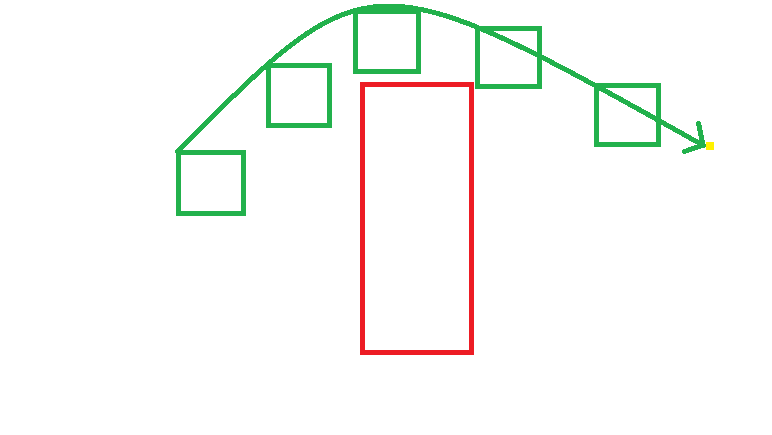
\includegraphics[scale=0.5]{images/path}
    \caption{}
    \label{fig:path}
\end{center}
\end{figure}

\subsection{Kitöltés}

(Ez sem biztos, hogy kész lesz).  Ennek a funkciónak az a lényege, hogy a felhasználó meg tudjon adni egy befoglaló téglalapot, amire megadja, hogy az egy kitöltött terület valamilyen ismétlődő képpel, és azt egyként kell kezelni, adódjon hozzá az adatbázis adataihoz. Ennek előnye, ha egy nagy pályát kiakarok tölteni teljesen fűvel(50x50), akkor ne kelljen kézzel berajzolgatni, hanem fill the map with picture funkció megoldja ezt helyettünk.

\subsection{Térkép mentés és visszaállítás}

(Ez sincs egyenlőre belerakva). A felhasználó szeretne térkép állapotokat menteni, majd esetleg visszaállítani a jelenlegi állapotokat egy későbbi állapotra. Naplózó művelet.

Save databasename mentésname;
Ezzel eltárolom ezt az állapotot.

Load mentésnév;
Ezt kiadva az aktuális állapot ez lesz. Javaból a kapcsolódáskor alapértelmezetten az utolsó mentett állapotot kérdezi le, viszont lehet állítani, hogy mely mentést szeretné folytatni.

\subsection{Entitások állapotának tárolása}

Szeretnénk egy olyan funkciót, hogy az egyes elemekről több információt is lehessen tárolni az adatbázisban, ez azért lenne fontos, mert így az üzleti logikát is lehetne tárolni benne. Ennek megoldása, hogy saját Classokat definiálhat a felhasználó, és a térkép adatok mellé üzleti logikát is tárolhat. A Classok saját típusdefiníciók, sémaleírók. Ez hasonló képpen működik mint Sql-ben a tábla definíció, csak itt nem táblák vannak, hanem objektumok.

\subsection{Rétegkezelés}

Különböző rétegeket tud kezelni az adatbázis. Ez azt jelenti, hogy például ütközés vizsgálatnál a különböző szinteken lévő elemeket nem ütközteti. Két alapértelmezett attribútumot bevezetése volt szükségszerű a feladat megoldásához:
-zindex
-zlayer

Ha két elem más szinten van, akkor a zlayer attribútumuk értéke eltérő. Különböző zlayereken lévő attribútumok között az ütközés vizsgálat nincs értelmezve. Ha azt szeretnénk, hogy minden adatbázisban tárolt objektum ütközhessen a többivel, akkor mindegyiknek a zlayer attribútumának az értéke meg kell, hogy egyezzen.
A kirajzolási sorrend fontos lehet a renderelésnél, a z-index pedig azt határozná meg, hogy melyiket mikor kell kirajzolni, mely elemek előtt vagy éppen után. A zindex attribútum olyan mint az id attribútum, minden Classnak van, és az adatbázismotor generálja vagy tölti fel értékkel. A felhasználó lekérdezheti, és módosíthatja ezen attribútumokat, viszont nem feltétlenül érdemes. A zindex értéket úgy tölti fel , hogy beszúrás alapján növeli a jelenlegi zindex értéket, majd azt adja hozzá. A Tile Editorban autómatikusan kitölti ennek az értékét.

A következő 4 attribútuma biztosan minden objektumnak van:
- id
- className
- zlayer
- zindex

\subsection{Távolság kiszámítása}

Szükség volt olyan lekérdezésre, aminek az eredménye az, hogy az 500 egységnél távolabb lévő elemeket listázza ki. A távolság számításnak több implementációja lenne(középpontok távolságát nézi, legközelebbi pontok távolságát, jobb felső sarok távolságát, stb..). Jelenlegi implementációban az ütközésvizsgálathoz az entitások bal felső sarkának koordinátáit használja.
\begin{sql}
SELECT mine
FROM azeroth
WHERE mine CLOSEST TO (10, 10) AND mine.distanceFrom(20, 20) > 30;
\end{sql}
A fenti lekérdezés kiválasztja azokat az elemeket a mapről, amelyek legközelebb vannak a (10,10) ponthoz, és a  (20,20) ponttól 30 ponttól nagyobb távra vannak.


A fekete vonal a távolság vektor.

